\documentclass[a4paper,man,natbib,11pt]{article}
\textwidth=7in
\textheight=9.5in
\topmargin=-1in
\headheight=0in
\headsep=.5in
\hoffset  -.85in

\usepackage[english]{babel}
\usepackage[utf8x]{inputenc}
\usepackage{amsmath}
\usepackage{setspace}
\usepackage{graphicx}
\usepackage{longtable}
\usepackage{caption}
\usepackage{subcaption}
%\usepackage{apacite}
\usepackage{tikz}
\usetikzlibrary{positioning,arrows.meta,quotes}
%\doublespacing
%\usepackage{lineno}
%\linenumbers
%packages for RSF portion
\usepackage{hyperref}
\usepackage{subfig}
\usepackage{float}
\usepackage{wrapfig}
\restylefloat{figure}

\title{Predicting Dementia using Machine Learning Methods}
\author{Peter Shewmaker, Nadia Mercado,Caroline Mills  }
\date{May 2020}

\begin{document}

\maketitle

\section{Introduction}

Dementia and other cognitive decline diseases are a serious financial and medical global concern. As such, in this paper we will test statistical classification methods from statistical learning methods, logistic regression, support vectors machines, and naive baye's. We will present the classification accuracy, specificity, sensitivity, and area under the ROC curve for all classifier methods. In addition, we will also explore modeling the "survival" curve or time to event models for dementia status. 

\section{Data}

The data was drawn from the National Alzheimer's Coordinating Center's Uniform Data Set. Located at the University of Washington, the National Alzheimer's Coordinating Center (NACC) was founded in 1999 by the National Institute on Aging, a division of the National Institutes of Health. The goal of the NACC is to develop and maintain databases of Alzheimer's related research data. The NACC Uniform Data Set is intended to be "the first and primary resource for researchers analyzing NACC clinical and demographic data".

The data contains one row for each clinic visit by a patient. It includes social, racial, educational demographic data, as well as cognitive test results, living situation, and smoking status. In order to use the data for the classification of dementia status, the last recorded visit by each patient included in the data was extracted.

However, the data had to be restructured differently for the survival analysis. For this, we needed to create the time to event variable. This was constructed subtracting the age of the participant from the first visit and the age of the participant at the first diagnosis of dementia or the age of the participant at the end of follow up (up to 12 years). The information for each participant was only kept at the initial diagnosis of dementia or at the last recorded visit. Lastly, we filtered for variables with more than 5\% of missing data, omitted any variables that have a summary variable available, and filtered for complete cases. The final dataset now only contained 20 variables.

\section{Classification by Test Scores - Peter Shewmaker}

Diagnosis of Alzheimer's disease and related dementias is often aided by the use of cognitive tests. The Uniform Data Set contains patient performance on a large variety of these cognitive tests. Some of these tests are owned by private companies or can only be administered by a medical professional. However, other tests could be simply administered by a loved one. 

The aim then was to develop a statistical learning model that could take in patient demographic information together with simple test score results that could theoretically be used for a home screening test for Alzheimer's diagnosis. Cognitive tests were chosen as predictors if they could be administered simply at home. 

Some of the cognitive tests chosen include: Logical Memory, which measures the number of components of a story a patient recalls immediately after being told the story. In the Animal/Vegetable test, the subject is asked to name as many animals (vegetables) as possible in 60 seconds. The Digit Span test involves giving a sequence of digits to a patient and asking them to repeat them, both in the forwards and backwards direction of the original sequence. The Trails test consists of a set of numbered (lettered) dots, and the patient is asked to connect the dots in numerical (alphabetical) order, the test is measured by the amount of time needed to complete the task.

\subsection{Logistic Regression}
Logistic regression is a commonly used model in predicting adverse outcomes in public health literature due to the ease of interpretation of coefficients and is a powerful classification algorithm. We will evaluate the predictive accuracy of the model In terms of overall classification accuracy, specificity, sensitivity, along with Random Forrest and Support Vector Machine(SVM). Of the 7,685 observations,  5,000 were classified as training data and the remaining 2,639 were classified as test data. 

First, we fit the logistic model to the training data. No transformations were preformed on any of the variables since we don't want to risk complicating the interpretation of the coefficients and odds's ratios associated to the transformed covariates. Stepwise selection was preformed with the Akaike information criterion (AIC) as a metric. We elected to include all variables since there was a minimal change in improvement. The fitted results were then applied to the test data. 

There are several methods to select a cut-off value. In many cases, c=0.50 is the most optimal choice, however this is not always the case especially for unbalanced data. For this model, we compared two cut-off classification methods 1) Youden Index which is max(Sensitivity+Specificity), a measurement considering both true positive rate and true negative rate and 2) the point closest to the top-left part of the plot with perfect sensitivity or specificity $min((1-sensitivities)^{2}+(1-specificities)^{2})$.The ROC curve below (receiver operating characteristic curve) shows the sensitivity and specificity trade-off for each cut-off value. 

\begin{figure}[h!]
\centering
  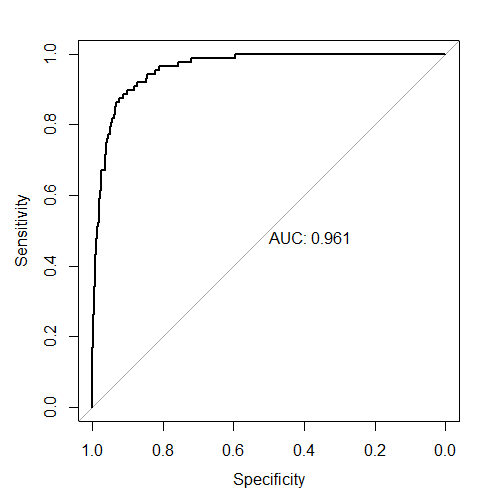
\includegraphics[width=0.5\textwidth]{roc_logistic.png}
  \caption{ROC for Testing Data}
\end{figure}

The results of the model were fitted to the test data. As we can see, when the classifier is set to 0.029 the model has the highest sensitivity and specificity.

\begin{figure}[h!]
\centering
  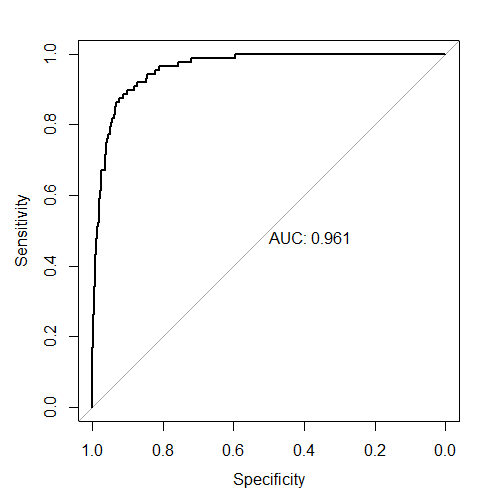
\includegraphics[width=0.5\textwidth]{roc_logistic.png}
  \caption{ROC for Testing Data}
\end{figure}


\subsection{Classification Tree}

The second model used to classify patient's dementia status was a classification tree. Of the 7,685 rows in the original data, 46 rows were excluded due to missing data. Then, of the remaining 7,639 rows, 5,000 were selected to form the training data. The remaining 2,639 rows were set aside to be the test set.

\begin{figure}[h!]
\centering
\begin{subfigure}{.5\textwidth}
  \centering
  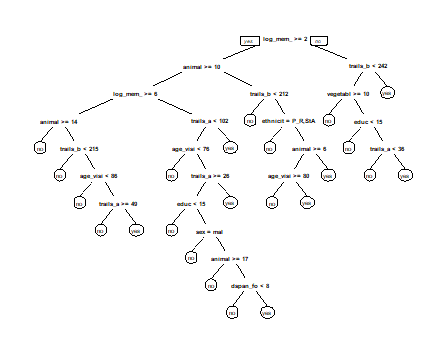
\includegraphics[width=\linewidth]{unpruned_tree.png}
  \caption{Unpruned Tree}
  \label{fig:sub1}
\end{subfigure}%
\begin{subfigure}{.5\textwidth}
  \centering
  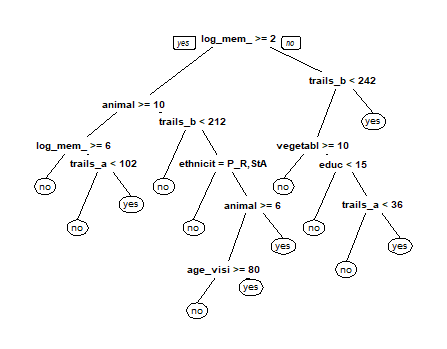
\includegraphics[width=\linewidth]{pruned_tree.png}
  \caption{Pruned Tree}
  \label{fig:sub2}
\end{subfigure}
\caption{Unpruned and Pruned Classification Trees}
\label{fig:test}
\end{figure}

The classification tree was created using the "rpart" package in R. Splits in the tree were made by the Gini index. The complexity parameter was chosen by repeated cross validation. The cross validation was performed using the R package "caret".

In Figure 1 you can see graphical depictions of both the pruned and unpruned trees. The tree was pruned by classification error. We see that the Logical Memory, Trails, and Animal/Vegetable tests are commonly chosen as places to split the tree.

\begin{figure}
\centering
\begin{subfigure}{.5\textwidth}
  \centering
  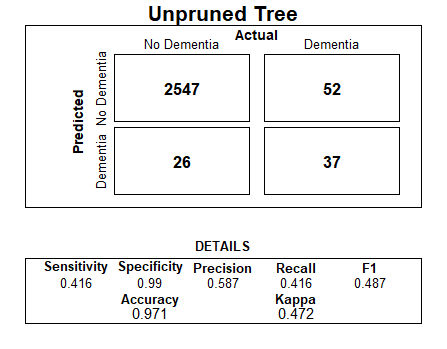
\includegraphics[width=\linewidth]{unpruned_confusion.png}
\end{subfigure}%
\begin{subfigure}{.5\textwidth}
  \centering
  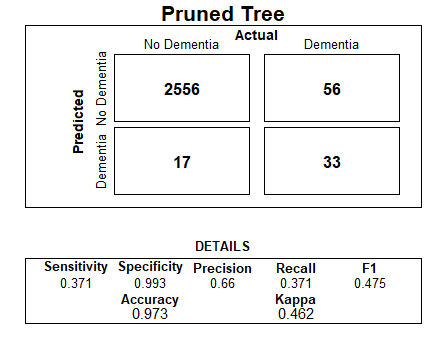
\includegraphics[width=\linewidth]{pruned_confusion.png}
\end{subfigure}
\caption{Unpruned and Pruned Classification Tree Results}
\label{fig:test}
\end{figure}

The comparison of the confusion matrices of the results of the unpruned and pruned tree can be found in Figure 2. We see that the accuracy of the tree was slightly improved after pruning. However, we see that the pruned tree has a lower sensitivity, and classifies correctly fewer of the patients who actually have dementia. 

\subsection{Random Forest with Downsampling}

Though the accuracy of each of the trees appears quite high, it is artificially inflated by the imbalance of the classes. Of the 2639 patients in the testing set, only 89 actually have Alzheimer's, which is 3.3\% of the test set. Therefore a decision tree that classified everyone as not having dementia would have a 96.7\% accuracy! 

Therefore we would like the model used to account for the unbalanced classes. We also see that the trees created in the previous section have a very low sensitivity, which would make it a poor diagnostic screening tool. By accounting for the unbalanced classes, we hope to improve the sensitivity of the classifier.

The method I used to account for the unbalanced classes is called \textit{downsampling}. In a downsampled random forest, instead of using a bootstrap sample from the entire training data set to create each tree, a bootstrap sample from the rare class is generated and a sample of the same size is generated from the common class are joined and used for the creation of the tree. Therefore each tree in the random forest model is built from a data set with the same number of observations in each class.

For some other statistical learning algorithms, the use of downsampling would require getting rid of a large amount of the data. However, since random forest uses resampling, the downsampling can be applied while still making use of the entirety of the training set.

\begin{figure}
\centering
\begin{subfigure}{.5\textwidth}
  \centering
  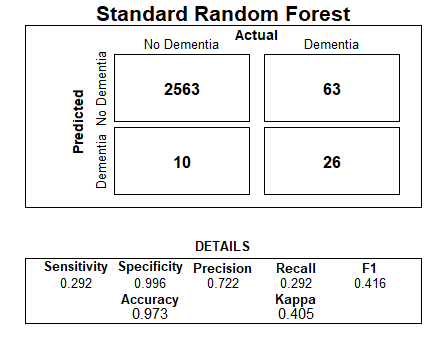
\includegraphics[width=\linewidth]{standard_rf.png}
\end{subfigure}%
\begin{subfigure}{.5\textwidth}
  \centering
  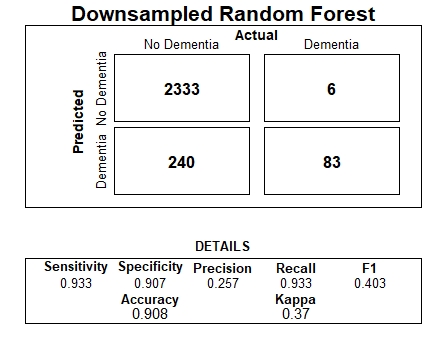
\includegraphics[width=\linewidth]{downsampled_rf.png}
\end{subfigure}
\caption{Standard and Downsampled Random Forest}
\label{fig:test}
\end{figure}

The random forest models were fit using the "caret" package. Cross validation was used to select optimal values for the number of trees and the "mtry" parameter.

The results of both the downsampled and the standard random forest models can be seen in Figure 3. Though the standard random forest model has a much higher accuracy (comparable to the classification trees), the downsampled random forest trades some accuracy for a drastic improvement in sensitivity. The sensitivity and specificity of the downsampled random forest are higher than 0.9, which means that it could be useful as a screening test. The algorithm was able to correctly identify 83 of the 89 patients who did in fact have dementia.

\subsection{Support Vector Machine}
The third model used to classify patient's dementia status was a support vector machine (SVM). This statistical learning model was selected since there is a clear margin of separation between classes and is  memory efficient. Of the 7,685 observations, 5,000 were selected as training data and the remaining 2,639 were selected as test data. 

\\~\\ SVM's are f
The e1071 library in R was used to put a SVM to the data. 

\section{Survival Analysis with Random Forests - Nadia Mercado}

The purpose of this project was to develop a model for dementia status using the NACC Alzheimer's data with the presence of the APOE genotype as our "treatment group". Random Survival Forests are a relatively new application which are an extension of Random Forest models to analyze time to event data. 

Random Survival Forests (RSF) use the log-rank splitting rule to identify variable importance with each observation using a Kaplan-Meier estimator within each terminal node for each time event. This model has been found to maintain a low prediction error, are uniformly consistent, and have a uniform approximating property in finite-sample settings. 

To develop the model, several R packages were explored. The first package ggRandomForests which is great for visually exploring survival models. This package also determines variable importance (VIMP) which is determined by the difference in the Out-of-Bag (OOB) prediction error before and after permutation. A large value indicates misspecification detracts from the predictive accuracy and a value close to zero or negative does not contribute to predictive accuracy or improves the predictive accuracy when the variable is misspecified. It can also determine variable importance by Minimal depth which assumes that variables with a high impact on the prediction are those that most frequently split nodes nearest to the root node and split the largest samples of the population. Another benefit of this package is the graphing capabilities where one can plot the predicted survival of each participant in the training or test data, look at variable dependence, partial dependence plots, and others. More information can be found in \href{https://arxiv.org/pdf/1612.08974.pdf}{Ehrlinger's paper} or the \href{https://cran.r-project.org/web/packages/ggRandomForests/index.html}{CRAN website}.

Another package is the ranger package which is commonly used for classification and regression random forests and can be extended to RSFs. This package uses the log-rank test for split criteria. Variable importance can be calculated as either VIMP or Minimal depth. It also calculates Harrell's C index, which can be described as a generalization of the ROC curve and can be used as a measure of prediction error where 1 - C-Index = Prediction Error. More information can be found in \href{https://arxiv.org/pdf/1508.04409.pdf}{Wright's and Zeigler's paper} or the \href{https://cran.r-project.org/web/packages/ranger/index.html}{CRAN website}.

In this section, we developed a RSF model and assessed variable importance by permutation for the ranger package and both permutation and minimal depth for the ggRandomForests package. Next, we assessed the top 5 variables summarized by all RSF models and assessed survival using a Cox Proportional Hazards model. We verified model assumptions and lastly compared this model with and without the APOE genotype using an ANOVA to see if we could still improve the model outside of the variables selected by RSF. The analysis for this portion of the paper was partially inspired by a \href{https://rviews.rstudio.com/2017/09/25/survival-analysis-with-r/}{blog post} in RStudio's website.

\subsection{Kaplan-Meier}

Prior to any analysis or assessment, we first plotted the Kaplan-Meier curve to get an overall view if there is a difference between the survival curves for participants with and without the APOE genotype. 

%KM comparison figure
\begin{figure}[h!]%
    \centering
    \subfloat[Overall Kaplan-Meier]{%
    {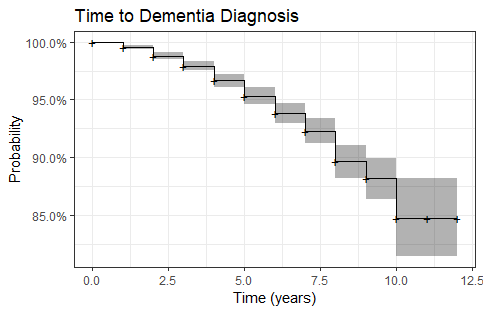
\includegraphics[width=5cm]{figures/KM1.PNG} }}%
    \qquad
    \subfloat[Kaplan-Meier by APOE genotype]{%
    {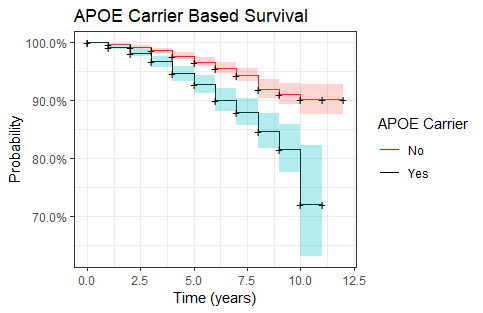
\includegraphics[width=5cm]{figures/KM2.PNG} }}%
    \caption{Comparison of Kaplain-Meier}%
    \label{fig:KM}%
\end{figure}

As seen in Figure \ref{fig:KM}, there does appear to be a difference in the survival curve for those with and without the APOE genotype.

\subsection{RSF model: ranger package}

While keeping the APOE genotype in mind, we can also fit a RSF model using the ranger package in R and check for variable importance by permutation. To be mindful of the page limitations, only the top 5 variables are represented in the Table \ref{ranger_vi}. 

% variable importance for ranger package
\begin{table}[ht]
\centering
% To place a caption
\caption{Ranger Package - Top 5 Variable Importance}
\begin{tabular}{rr}
  \hline
 & Importance \\ 
  \hline
cdr\_global & 0.12 \\ 
  log\_mem\_imm & 0.03 \\ 
  trails\_b & 0.01 \\ 
  animal & 0.01 \\ 
  vegetable & 0.01 \\ 
   \hline
\end{tabular}
\label{ranger_vi}
\end{table}

We observe that cdr\_global (a summary measurement of cognition) and log\_mem\_imm (a measure of cognition by retelling a story) are the two top variables identified by the model. In addition, the Hartnell's index and prediction error are available in Table \ref{ranger_stat}.

%C index and pred error
\begin{table}[ht]
\centering
\caption{Ranger Package - Summary Statistics}
\begin{tabular}{rrr}
  \hline
 & C Index & Prediction Error \\ 
  \hline
1 & 0.75 & 0.25 \\ 
   \hline
\end{tabular}
\label{ranger_stat}
\end{table}

\subsection{RSF model: ggRandomForests package}

We can get really great visuals from the ggRandomForests package in R. We can easily plot the prediction for each individual where the red lines represented the censored data (participants that did not experience the event of interest) and the uncensored data (participants that did experience the event of interest. This is illustrated in Figure \ref{fig:RSF_pred} 

%all prediction graph
\begin{figure}[h!]%
    \centering
    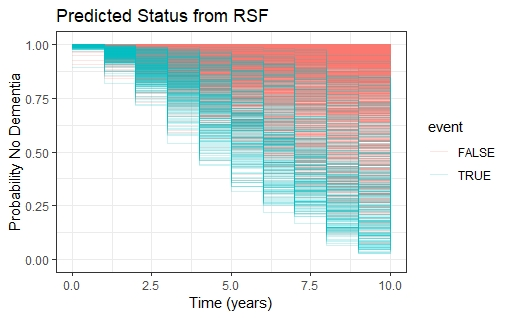
\includegraphics[width=0.5\textwidth]{figures/Predicted_Individual_RSF.jpeg}
    \caption{RSF Individual Predictions}%
    \label{fig:RSF_pred}%
\end{figure}

We can also check the ggRandomForests package if VIMP or Minimal depth are calculated differently than the ranger package and is illustrated in Figure \ref{fig:ggVI}. 

%ggRandomForest comparison figure
\begin{figure}[h!]%
    \centering
    \subfloat[Permutation]{%
    {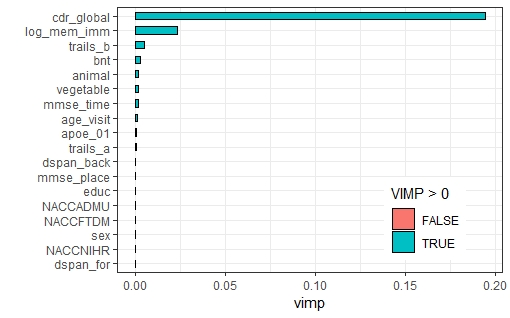
\includegraphics[width=5cm]{figures/VI_SRF.jpeg} }}%
    \qquad
    \subfloat[Minimal Depth]{%
    {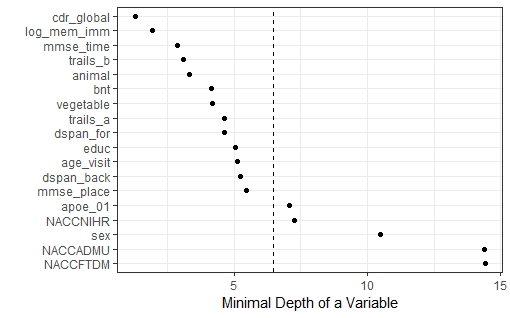
\includegraphics[width=5cm]{figures/MD_SRF.jpeg} }}%
    \caption{Comparison of Variable Importance}%
    \label{fig:ggVI}%
\end{figure}

\subsection{Cox Proportional Hazards model: survival package}

From this, we can take the top 5 variables that we see in both packages and fit into a Cox Proportional Hazards model as shown in Table \ref{cox_coef}. This model also includes the APOE genotype although it was not ranked high by permutation or Minimal depth. For all models, the assumption of proportionality was not violated (data not shown).   

\begin{table}[ht]
\centering
\caption{Cox Model: Surv(time,status)~apoe+cdr+mem+trails\_b+animal+bnt}
\begin{tabular}{rrrrrr}
  \hline
 & coef & exp.coef. & se.coef. & z & Pr($>$$|z|$) \\ 
  \hline
apoe & 0.38 & 1.47 & 0.13 & 2.95 & 0.00 \\ 
  cdr\_global & 1.58 & 4.84 & 0.14 & 11.62 & 0.00 \\ 
  log\_mem\_imm & -0.18 & 0.83 & 0.02 & -11.41 & 0.00 \\ 
  trails\_b & 0.00 & 1.00 & 0.00 & 1.98 & 0.05 \\ 
  animal & -0.05 & 0.95 & 0.02 & -3.04 & 0.00 \\ 
  bnt & 0.02 & 1.02 & 0.01 & 1.81 & 0.07 \\ 
   \hline
\end{tabular}
\label{cox_coef}
\end{table}


Lastly, we can fit an ANOVA to see if adding the APOE genotype predictor improves model fit (Table \ref{anova}). For this, we are comparing the Cox model with and without the addition of the APOE genotype. Model 1 does not include the APOE genotype and Model 2 does include the APOE genotype. 

%anova for cox models
\begin{table}[ht]
\centering
% To place a caption
\caption{Hypothesis Testing: testing the effect of the APOE genotype}
\begin{tabular}{lrrrr}
  \hline
 & loglik & Chisq & Df & P($>$$|$Chi$|$) \\ 
  \hline
1 & -1631.74 &  &  &  \\ 
  2 & -1627.42 & 8.64 & 1 & 0.0033 \\ 
   \hline
\end{tabular}
\label{anova}
\end{table}

It appears as if the addition of the APOE genotype does improve model fit even though the RSF models did not rank APOE in the top 5 variables. Lastly, we can compare the survival curves for each of the models: Kaplan-Meier, Cox Proprotional Hazards, and RSF (Figure \ref{fig:all_curves}. 

%all prediction graph
\begin{figure}[h!]%
    \centering
    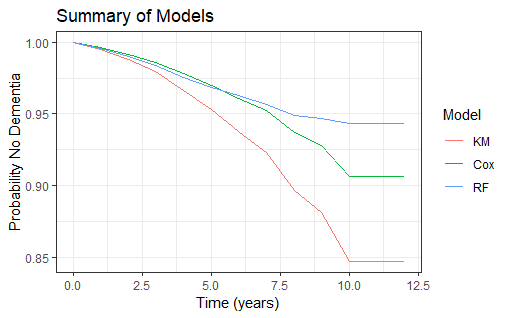
\includegraphics[width=0.5\textwidth]{figures/Summary_curves.png}
    \caption{Summary of Survival Curves}%
    \label{fig:all_curves}%
\end{figure}

\subsection{Conclusion}

Random Survival Forests are an interesting and powerful tool to model survival curves and can eliminate some of the challenges that a linear or parametric model may have. However, there are some limitations to this analysis in R. Currently, there is little support for tuning the parameters in the RSF models. Although caret is a popular choice for this, Tidymodels is currently exploring the possibility to allow for turning in RSFs. In addition, RSFs are currently not capable of adjusting for time varying coefficients, but can still be assessed manually. Lastly, RSFs should not be used to model survival analysis and should be used as a tool to enhance our understanding and for model prediction, but interpretation may be difficult. Therefore, we should still explore other avenues of survival modeling such as a Cox Proportional Hazards model.

\end{document}
